\documentclass[11pt,a4paper]{article}
\newcommand{\simname}{Extended Shot Peening Coverage Simulator}
\usepackage[utf8]{inputenc}
\usepackage[T1]{fontenc}
\usepackage[sc]{mathpazo}
\linespread{1.05}
\usepackage[english]{babel}
\usepackage[margin=2.2cm]{geometry}
\usepackage{amsmath,amssymb}
\usepackage[locale=UK,per-mode=symbol]{siunitx}
\usepackage{booktabs,array,tabularx,longtable}
\usepackage{graphicx}
\usepackage{tikz}
\usetikzlibrary{arrows.meta,decorations.pathreplacing,calc}
\usepackage{xcolor}
\usepackage[hidelinks]{hyperref}
\usepackage{enumitem}
\usepackage{tcolorbox}
\usepackage{float}
\usepackage[font=small,labelfont=bf]{caption}
\usepackage{subcaption}
\usepackage{fancyhdr}
\usepackage{multicol}

\definecolor{bleu}{HTML}{1F5A96}
\definecolor{orange}{HTML}{D4621C}
\definecolor{vert}{HTML}{2E8B57}
\definecolor{rouge}{HTML}{E5484D}
\newtcolorbox{keybox}[1][]{colback=bleu!5,colframe=bleu,boxrule=0.6pt,arc=2pt,left=6pt,right=6pt,top=4pt,bottom=4pt,#1}
\newtcolorbox{trybox}[1][]{colback=orange!6,colframe=orange,boxrule=0.6pt,arc=2pt,left=6pt,right=6pt,top=4pt,bottom=4pt,#1}
\newcommand{\E}{\mathbb{E}}
\newcommand{\dX}{\Delta X}
\newcommand{\ui}[1]{\textsf{#1}}   % name of a control or a readout on the page
\setlength{\tabcolsep}{5pt}
\renewcommand{\arraystretch}{1.15}

\pagestyle{fancy}
\fancyhf{}
\fancyhead[L]{\small Dr Régis Kubler, Arts et Métiers Institute of Technology}
\fancyhead[R]{\small\simname}
\fancyfoot[C]{\small\thepage}
\renewcommand{\headrulewidth}{0.4pt}
\setlength{\headheight}{14pt}
\setlength{\parskip}{3pt}
\usepackage{newunicodechar}
\newunicodechar{λ}{\ensuremath{\lambda}}
\newunicodechar{Σ}{\ensuremath{\Sigma}}
\newunicodechar{Δ}{\ensuremath{\Delta}}
\newunicodechar{δ}{\ensuremath{\delta}}
\newunicodechar{τ}{\ensuremath{\tau}}
\newunicodechar{σ}{\ensuremath{\sigma}}
\newunicodechar{η}{\ensuremath{\eta}}
\newunicodechar{α}{\ensuremath{\alpha}}
\newunicodechar{φ}{\ensuremath{\varphi}}
\newunicodechar{ζ}{\ensuremath{\zeta}}
\newunicodechar{²}{\ensuremath{^2}}
\newunicodechar{³}{\ensuremath{^3}}
\newunicodechar{−}{\ensuremath{-}}
\newunicodechar{·}{\ensuremath{\cdot}}
\newunicodechar{×}{\ensuremath{\times}}
\newunicodechar{≈}{\ensuremath{\approx}}
\newunicodechar{≥}{\ensuremath{\geq}}
\newunicodechar{≤}{\ensuremath{\leq}}
\newunicodechar{→}{\ensuremath{\rightarrow}}
\newunicodechar{°}{\ensuremath{^\circ}}
\newunicodechar{µ}{\ensuremath{\mu}}
\newunicodechar{…}{\ldots}
\newunicodechar{ṁ}{\ensuremath{\dot m}}
\newunicodechar{Ṅ}{\ensuremath{\dot N}}
\newunicodechar{₀}{\ensuremath{_0}}
\newunicodechar{₉}{\ensuremath{_9}}
\newunicodechar{₈}{\ensuremath{_8}}
\newunicodechar{₅}{\ensuremath{_5}}


\title{\textbf{Extended Shot Peening Coverage Simulator}\\[3pt]
\large User and theory guide: coverage of a flat part swept by raster paths}
\author{Dr Régis Kubler\\ Arts et Métiers Institute of Technology\\[4pt]
\small Developed with the assistance of Claude Opus 5.5 (Anthropic), November 2026}
\date{Guide for simulator version 2.3 (22 November 2026)\\ \url{https://rkubler.github.io/extended-simulator/}}

\begin{document}
\maketitle
\thispagestyle{fancy}

\begin{abstract}
\noindent This guide explains the Extended Shot Peening Coverage Simulator. It starts with the basic idea and a first experiment, then explains the model of a part swept by back-and-forth lines (rasters) at 0° and 90°, the three jet profiles, the stripes, the average and stripe-corrected models, every parameter, every result and chart displayed, the specified coverages above 100\,\% (treatment times) of NF~L~06-832, and the validation of the page.
\end{abstract}

\tableofcontents

\section{The idea in one page}

\paragraph{From a point to a whole part.} The Shot Peening Coverage Simulator follows a small area under a jet that passes over it again and again: coverage there obeys $\tau=100\,(1-e^{-Kn})$. On a real part the nozzle follows a \emph{raster}: parallel lines travelled back and forth, separated by a step $\delta$, sometimes followed by a second raster at 90°. The jet, of width $\dX$, overlaps neighbouring lines. When $\dX$ is not a whole multiple of $\delta$, some points are crossed by more lines than others, and the impacts pile up in \emph{stripes} parallel to the path.

\paragraph{What the page computes.} For each point $(x,y)$ of the part it computes the expected number of impacts $\lambda(x,y)$, then the local coverage $\tau=1-e^{-\lambda}$. It shows the map of the part, a cross-section across the lines, the mean, minimum and maximum coverage, and compares them with two models:
\begin{itemize}[nosep]
\item the \textbf{average model} $1-e^{-K_\delta n}$, which spreads the impacts evenly and ignores the stripes;
\item the \textbf{stripe-corrected model}, which averages the local coverage over the stripes.
\end{itemize}

\begin{trybox}
\textbf{First experiment.} The page opens with the reference media and jet of the Excel model ($K=0.337$ for one pass along one line), a Gaussian jet of $\dX=\SI{20}{mm}$, a step $\delta=\SI{15}{mm}$ and 3 rasters at 0° alternating with 3 at 90° on a $100\times\SI{100}{mm}$ part. Press \ui{Play} and watch the stripes appear, then cross. Results (\ui{Run all}):
\begin{itemize}[nosep]
\item mean coverage \SI{92.9}{\percent}, between \SI{87.7}{\percent} in the weakest point and \SI{96.3}{\percent} in the strongest;
\item average model \SI{93.2}{\percent}: slightly optimistic, because it ignores the stripes;
\item 98\,\% (the base time) needs 8.9 rasters, full coverage (100\,\%, NF~L~06-832) 11.2 rasters.
\end{itemize}
Then set the step to \SI{10}{mm}: the stripes almost vanish (\SI{2.8}{\percent}) and both models agree.
\end{trybox}

\section{The screen}

\begin{figure}[H]
\centering
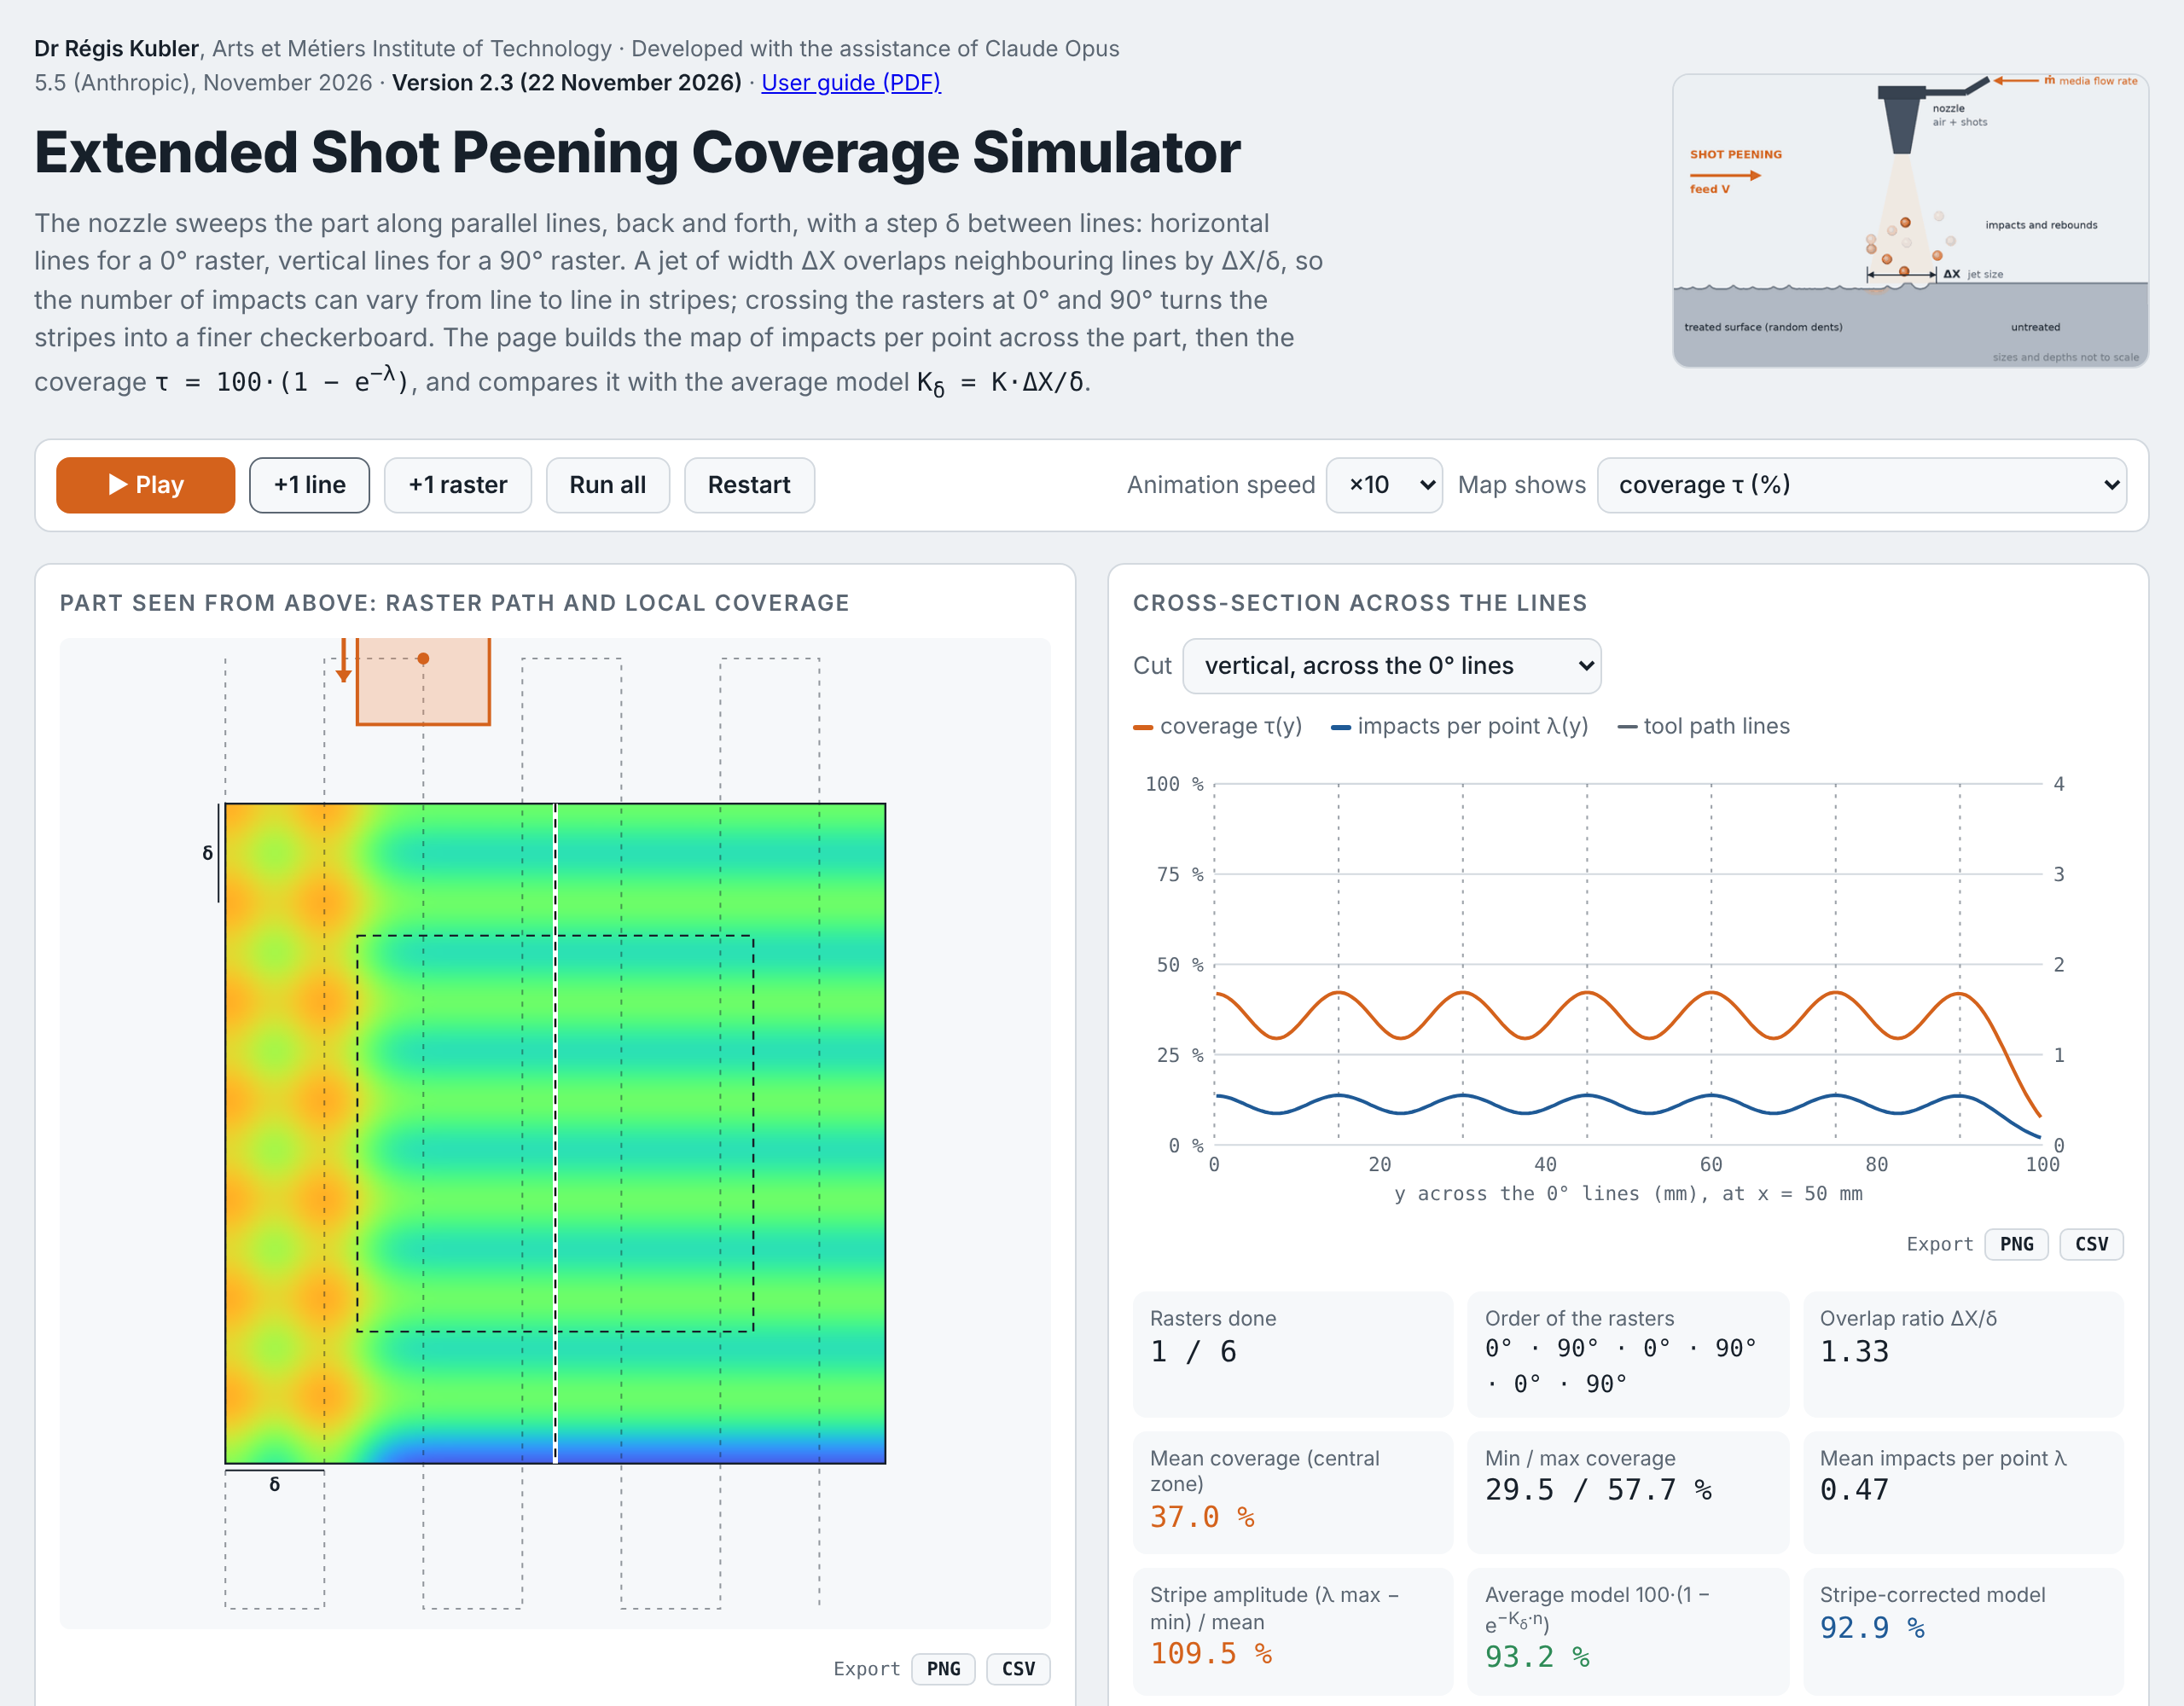
\includegraphics[width=\linewidth]{img/overview.png}
\caption{The page during the second raster (90°, vertical lines). Left: the part seen from above, with the path of the current raster, the jet footprint (orange square), the central zone used for statistics (dashed) and the cross-section line. Right: cross-section and readouts.}
\end{figure}

\paragraph{Toolbar.}
\begin{description}[leftmargin=2.6cm,style=nextline,itemsep=2pt]
\item[\ui{Play / Pause}] runs or stops the animation (\ui{Replay} at the end).
\item[\ui{+1 line}] travels exactly one more line and stops.
\item[\ui{+1 raster}] completes the current raster and stops.
\item[\ui{Run all}] computes all the rasters at once.
\item[\ui{Restart}] clears the part.
\item[\ui{Animation speed}] $\times0.5$ to $\times10$; it changes only the drawing speed.
\item[\ui{Map shows}] coverage $\tau$ (\%), impacts per point $\lambda$, or local coverage (NF~L~06-832), which can exceed 100\,\% (Section~\ref{sec:above}).
\end{description}

\paragraph{Export.} Under every figure, \ui{Export PNG} saves the figure exactly as it is shown at that instant (also during the animation) as a PNG image: map of the part, side and front views of the nozzles, cross-section and the two charts. \ui{CSV} saves the data behind it as a CSV file (comma separated, UTF-8, readable by Excel, Python or Matlab): the map as shown (coverage, $\lambda$ or NF coverage at every point of the grid), the cross-section, the coverage versus the number of rasters (both models and the simulated points) and the one-raster coverage versus the step. The file names contain the date and time.

\paragraph{Panels.}
\begin{enumerate}[nosep]
\item \textbf{Part seen from above}: the map, its colour scale (rainbow from untreated grey to red) and the hover readout. Clicking the map moves the cross-section line. Below it, the \textbf{side view of the nozzles along the current line}: a section in the plane of the path and the normal, with the part, its edges and the overtravel, the nozzle (or the two nozzles) tilted by $\theta_1$ and $\theta_2$ with the normal and the angles, the jets, their footprints $\dX/\cos\theta_k$ along the path and the direction of travel. The stand-off distance is not to scale.
\item \textbf{Cross-section across the lines}: $\tau$ (orange, left axis) and $\lambda$ (blue, right axis) along a vertical cut (across the 0° lines) or a horizontal cut (across the 90° lines), with the positions of the lines as dotted marks. Below it, the main readouts.
\item \textbf{Coverage versus number of rasters}: both models, the simulated points, the markers for 98\,\%, 100\,\% and the specified coverage, and the time readouts.
\item \textbf{One-raster coverage versus step $\delta$}: the effect of the step for a single raster.
\item \textbf{Parameters}.
\item \textbf{How the extended model works}: the calculation chain with the current values.
\end{enumerate}

\section{Summary of the equations}

\begin{keybox}
\textbf{Local coverage.} At each point of the part,
\begin{equation}
\tau(x,y)=100\,\bigl(1-e^{-\lambda(x,y)}\bigr),\qquad
\lambda(x,y)=\frac{a\,\dot N}{V}\Bigl[\sum_{\text{0° lines}} g(y-y_j)+\sum_{\text{90° lines}} g(x-x_j)\Bigr],
\label{eq:lambda}
\end{equation}
where $a$ is the mean dent area, $\dot N$ the number of shots per second, $V$ the traverse speed and $g$ the jet profile across the line ($\int g=1$).

\smallskip
\textbf{Average model} (ignores the stripes): with $n$ rasters in total,
\begin{equation}
\bar\tau_{\text{avg}}=100\,\bigl(1-e^{-K_\delta n}\bigr),\qquad K_\delta=\frac{a\,\dot N}{V\,\delta}=K\,\frac{\dX}{\delta}.
\label{eq:avg}
\end{equation}

\textbf{Stripe-corrected model}: the mean of the local coverage,
\begin{equation}
\bar\tau=100\,\Bigl(1-\bigl\langle e^{-\lambda_{0}(y)}\bigr\rangle\,\bigl\langle e^{-\lambda_{90}(x)}\bigr\rangle\Bigr)\;\le\;\bar\tau_{\text{avg}},
\label{eq:corr}
\end{equation}
where $\lambda_0$ and $\lambda_{90}$ are the impacts brought by the 0° and 90° rasters and $\langle\cdot\rangle$ is the mean over the central zone of the part (the zone used for the statistics, at a distance $\dX$ from the edges).

\smallskip
\textbf{Stripes of a Gaussian jet} ($\sigma_j=\dX/4$): the relative amplitude of $\lambda$ for one raster is
\begin{equation}
\frac{\lambda_{\max}-\lambda_{\min}}{\bar\lambda}\simeq 4\,e^{-2\pi^2(\sigma_j/\delta)^2},
\end{equation}
which is below \SI{3}{\percent} for $\delta\le\dX/2$.
\end{keybox}

\section{Recall of the original model}\label{sec:recall}

The jet throws a media flow rate $\dot m$ of shots of density $\rho$. For shots of diameter $D$ following a log-normal distribution of mass median $D_{50}$ and spread $\sigma$, the mean mass of one shot involves the mean of the cube of the diameter:
\begin{equation}
\bar m_p=\rho\,\frac{\pi}{6}\,\E[D^3],\qquad \E[D^3]=D_{50}^3\,e^{-4.5\,\sigma^2},\qquad \dot N=\frac{\dot m}{\bar m_p}.
\end{equation}
$\E[D^3]$ is the mean over all shots of $D^3$, each shot counting once. It is larger than the cube of the mean diameter because large shots weigh much more. For identical shots ($\sigma=0$), $\E[D^3]=D^3$. From a sieve analysis with mass fractions $w_i$ in classes of diameter $D_i$, $\E[D^3]=\sum w_i/\sum(w_i/D_i^3)$.

With dents proportional to the shot diameter, $r=c\,D$ with $c=r_{50}/D_{50}$, the mean dent area is
\begin{equation}
a=\pi\,c^2\,\E[D^2],\qquad \E[D^2]=D_{50}^2\,e^{-4\sigma^2}.
\end{equation}
For one line of width $\dX$ swept at speed $V$, the mean number of impacts per point after $n$ passes is $Kn$ with
\begin{equation}
K=\frac{a\,\dot N}{V\,\dX},
\end{equation}
and the coverage is $\tau=100(1-e^{-Kn})$. With the default values of the page ($\dot m=\SI{1.5}{kg/min}$, $\rho=\SI{2.2}{g/cm^3}$, $D=\SI{150}{\micro m}$, $\sigma=0$, $r=\SI{10}{\micro m}$, $\dX=\SI{20}{mm}$, $V=\SI{300}{mm/s}$): $\bar m_p=\SI{3.89}{\micro g}$, $\dot N=\num{6.43e6}$ shots/s, $a=\SI{3.14e-4}{mm^2}$ and $K=0.337$, i.e.\ \SI{28.6}{\percent} coverage after one pass.

\section{Raster paths}

\subsection{Geometry}

\begin{figure}[H]
\centering
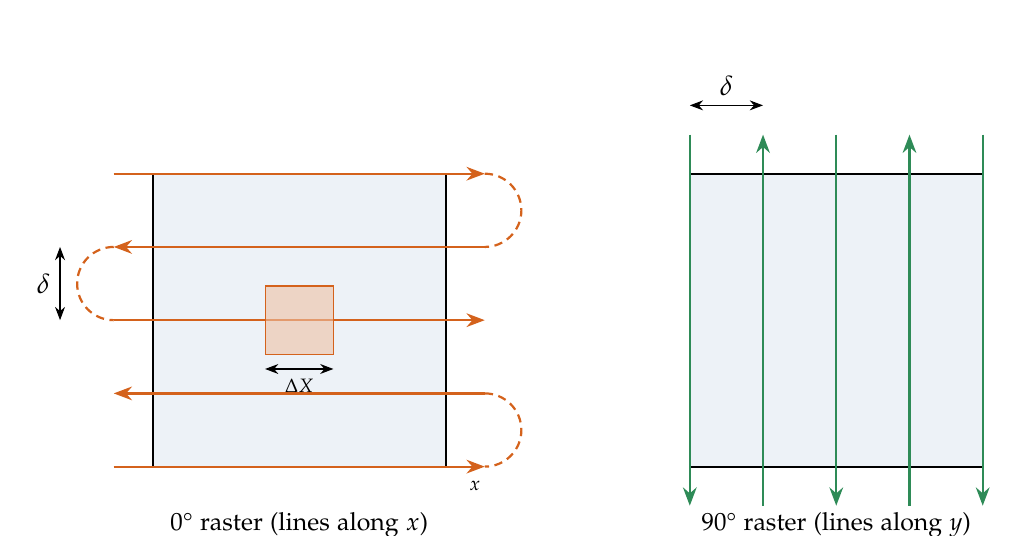
\begin{tikzpicture}[scale=0.62,>=Stealth]
% part 0°
\begin{scope}
\fill[bleu!8] (0,0) rectangle (6,6);
\draw[thick] (0,0) rectangle (6,6);
\foreach \y/\d in {6/1,4.5/-1,3/1,1.5/-1,0/1}{
  \ifnum\d=1 \draw[orange,thick,->] (-0.8,\y) -- (6.8,\y); \else \draw[orange,thick,->] (6.8,\y) -- (-0.8,\y); \fi}
\foreach \y in {6,1.5}{\draw[orange,thick,densely dashed] (6.8,\y) arc (90:-90:0.75);}
\foreach \y in {4.5}{\draw[orange,thick,densely dashed] (-0.8,\y) arc (90:270:0.75);}
\draw[<->] (-1.9,4.5) -- (-1.9,3) node[midway,left] {$\delta$};
\fill[orange!40,opacity=.6] (2.3,2.3) rectangle (3.7,3.7);
\draw[orange] (2.3,2.3) rectangle (3.7,3.7);
\draw[<->] (2.3,2.0) -- (3.7,2.0) node[midway,below] {\scriptsize$\Delta X$};
\node at (3,-1.2) {\small 0° raster (lines along $x$)};
\node[font=\scriptsize] at (6.6,-0.4) {$x$};
\end{scope}
% part 90°
\begin{scope}[xshift=11cm]
\fill[bleu!8] (0,0) rectangle (6,6);
\draw[thick] (0,0) rectangle (6,6);
\foreach \x/\d in {0/1,1.5/-1,3/1,4.5/-1,6/1}{
  \ifnum\d=1 \draw[vert,thick,->] (\x,6.8) -- (\x,-0.8); \else \draw[vert,thick,->] (\x,-0.8) -- (\x,6.8); \fi}
\draw[<->] (0,7.4) -- (1.5,7.4) node[midway,above] {$\delta$};
\node at (3,-1.2) {\small 90° raster (lines along $y$)};
\end{scope}
\end{tikzpicture}
\caption{Raster paths. The nozzle travels back and forth along parallel lines separated by the step $\delta$, and keeps firing during the turnarounds, which take place outside the part (overtravel). A 0° raster sweeps lines along $x$, a 90° raster lines along $y$. The orange square is the jet footprint $\dX\times\dX$.}
\label{fig:raster}
\end{figure}

The part is a rectangle of length $W$ along $x$ and width $H$ along $y$. A 0° raster has lines at $y_j=o+j\delta$, $j=0,1,\dots$ with $y_j\le H$, swept alternately in the $+x$ and $-x$ directions; a 90° raster has lines at $x_j=o+j\delta$ swept along $y$. The offset $o$ is zero, or $\delta/2$ for every other raster of the same direction when the option ``half step every other raster'' is selected. Each line extends beyond the part by an overtravel equal to the reach of the jet plus \SI{2}{\percent} of the line length, so that the ends of the part are treated like its middle. The user chooses the number $n_0$ of 0° rasters, the number $n_{90}$ of 90° rasters and their order: alternate (0°, 90°, 0°, 90°, \dots) or all 0° rasters first.

\subsection{Jet profile}

The jet is described by its profile $g$ across the line, normalised so that $\int g\,\mathrm{d}u=1$. The footprint is taken as the product $g(x)\,g(y)$, which is exact for an axisymmetric Gaussian jet. Three profiles are available (Fig.~\ref{fig:profile}):
\begin{align}
\text{uniform:}\quad & g(u)=\frac{1}{\dX}\ \text{ for } |u|<\frac{\dX}{2},\ 0 \text{ otherwise};\\
\text{Gaussian:}\quad & g(u)=\frac{1}{\sqrt{2\pi}\,\sigma_j}\,e^{-u^2/(2\sigma_j^2)}=\frac{4}{\sqrt{2\pi}\,\dX}\,e^{-8u^2/\dX^2},\qquad \sigma_j=\frac{\dX}{4};\\
\text{flattened Gaussian:}\quad & g(u)=\frac{1}{2w\,\Gamma(1+1/p)}\,e^{-|u/w|^p},\qquad w=\frac{\dX/2}{2^{1/p}},\quad p\ge2.
\label{eq:flat}
\end{align}
With $\sigma_j=\dX/4$, the jet size $\dX$ spans $\pm2\sigma_j$ and contains \SI{95.4}{\percent} of the shots; the intensity at the edges $\pm\dX/2$ is \SI{13.5}{\percent} of the peak, and the peak is $1.596/\dX$, about 1.6 times that of the uniform jet. The page ``Jet Profile Explained'', opened by the \textsf{i} button next to the profile choice, plots the three profiles and their overlap.

\paragraph{Flattened Gaussian.} Measured intensity profiles of air-blast nozzles are bell-shaped but can be flatter on top than a Gaussian; a study of a direct-pressure air-blast nozzle fitted them with a modified Gaussian that has an exponent controlling the flatness \cite{mt2019}. The flattened (or super-) Gaussian of Eq.~\eqref{eq:flat} offers this freedom with one extra parameter, the exponent $p$:
\begin{itemize}[leftmargin=*]
\item $\Gamma$ is the gamma function; the factor $1/(2w\Gamma(1+1/p))$ makes $\int g=1$, so all three profiles carry the same number of shots and the same media flow rate.
\item $w$ is chosen so that $g(\pm\dX/2)=e^{-2}\,g(0)$, i.e.\ \SI{13.5}{\percent} of the peak, exactly as for the Gaussian. $\dX$ therefore keeps the same meaning for both bell-shaped profiles.
\item $p=2$ gives back the Gaussian with $\sigma_j=\dX/4$; as $p$ grows the top flattens and the sides steepen, and the profile tends to the uniform jet. For $p=4$ the peak is $1.312/\dX$ and \SI{98.3}{\percent} of the shots land inside $\dX$ (\SI{95.4}{\percent} for the Gaussian, \SI{100}{\percent} for the uniform jet).
\item In the page, $p$ ranges from 2 to 20 (default 4) and is used only when the flattened profile is selected.
\end{itemize}

\begin{figure}[H]
\centering
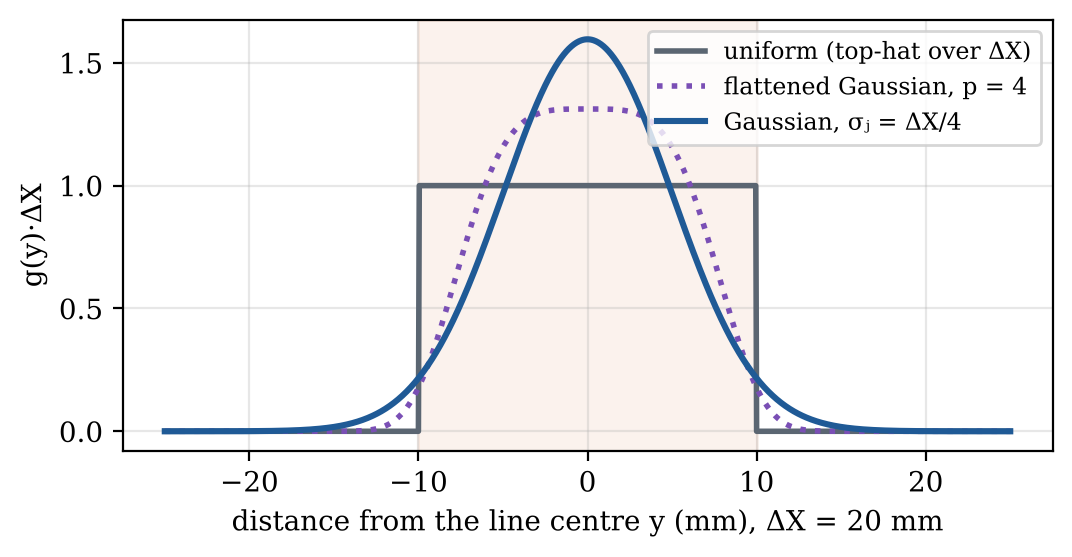
\includegraphics[width=0.66\linewidth]{img/profile.png}
\caption{Uniform, Gaussian and flattened Gaussian ($p=4$) jet profiles across the line for $\dX=\SI{20}{mm}$. All carry the same number of shots (same area under the curve). The shaded band is the jet size $\dX$.}
\label{fig:profile}
\end{figure}

\section{Impacts per point and stripes}

\subsection{Expected number of impacts per point}

When the nozzle passes once along a long line at $y_j$, a point at distance $u=y-y_j$ receives on average
\begin{equation}
\lambda_{\text{line}}(u)=\frac{a\,\dot N}{V}\,g(u)
\end{equation}
impacts: the jet throws $\dot N/V$ shots per millimetre of travel, a fraction $g(u)\,\mathrm{d}u$ of them land in a strip of width $\mathrm{d}u$, and each one covers an area $a$. Summing over all lines of all rasters gives Eq.~\eqref{eq:lambda}. The 0° rasters bring a term that depends on $y$ only, the 90° rasters a term that depends on $x$ only:
\begin{equation}
\lambda(x,y)=\lambda_0(y)+\lambda_{90}(x).
\end{equation}

\subsection{Average over the part: the average model}

For one raster, the integral of $\sum_j g(y-j\delta)$ over one step $\delta$ is 1, so the mean of $\lambda$ over the part is
\begin{equation}
\bar\lambda=n\,\frac{a\,\dot N}{V\,\delta}=n\,K_\delta,\qquad K_\delta=K\,\frac{\dX}{\delta},
\end{equation}
with $n=n_0+n_{90}$. Each point is crossed on average by $\dX/\delta$ lines per raster, hence the factor. This mean is exact whatever the stripes. The average model then assumes that every point receives $\bar\lambda$ impacts, which gives Eq.~\eqref{eq:avg}. It reduces to the original model $1-e^{-Kn}$ for $\delta=\dX$.

The average model does \emph{not} give the coverage of one stripe. It is the coverage the part would have if the impacts were spread evenly. Because $1-e^{-\lambda}$ is concave, Jensen's inequality gives
\begin{equation}
\bigl\langle 1-e^{-\lambda}\bigr\rangle\le 1-e^{-\langle\lambda\rangle},
\end{equation}
so the average model is an upper bound of the true mean coverage: it is optimistic whenever there are stripes.

\subsection{Stripe-corrected model}

The stripe-corrected model takes the mean of the local coverage, $\bar\tau=\langle 1-e^{-\lambda}\rangle$, over the central zone of the part, with the lines actually travelled. The page evaluates it numerically on 600 points across the zone, separately for the 0° lines (across $y$) and the 90° lines (across $x$). The chart ``one-raster coverage versus step'' uses instead the mean over one period $2\delta$ (two steps, to include the half-step offset), which describes an infinitely large part.

\paragraph{Uniform jet: closed form.} With a top-hat jet a point is crossed by either $m_0=\lfloor \dX/\delta\rfloor$ or $m_0+1$ lines per raster. The stripes crossed $m_0+1$ times occupy a fraction $f=\dX/\delta-m_0$ of the surface. Each kind of stripe has its own coverage, and the mean is
\begin{equation}
\bar\tau=1-(1-f)\,e^{-K m_0 n}-f\,e^{-K(m_0+1)n}.
\end{equation}
The weakest stripe has the coverage $1-e^{-Km_0n}$, the strongest $1-e^{-K(m_0+1)n}$. There are no stripes when $\dX/\delta$ is a whole number ($f=0$), and untreated strips remain when $\delta>\dX$ ($m_0=0$).

\paragraph{Gaussian jet: stripe amplitude.} By Poisson's summation formula,
\begin{equation}
\sum_j g(y-j\delta)=\frac{1}{\delta}\Bigl[1+2\sum_{k\ge1} e^{-2\pi^2k^2\sigma_j^2/\delta^2}\cos\frac{2\pi k y}{\delta}\Bigr].
\end{equation}
The first harmonic dominates, so $\lambda$ oscillates around its mean with a relative peak-to-peak amplitude $\simeq 4\,e^{-2\pi^2(\sigma_j/\delta)^2}$: \SI{2.9}{\percent} for $\delta=\SI{10}{mm}$, \SI{44.6}{\percent} for $\delta=\SI{15}{mm}$ and \SI{182}{\percent} for $\delta=\SI{25}{mm}$ (with $\dX=\SI{20}{mm}$). Below $\delta=\dX/2=2\sigma_j$ a Gaussian jet gives practically uniform coverage (Fig.~\ref{fig:stripes}).

\begin{figure}[H]
\centering
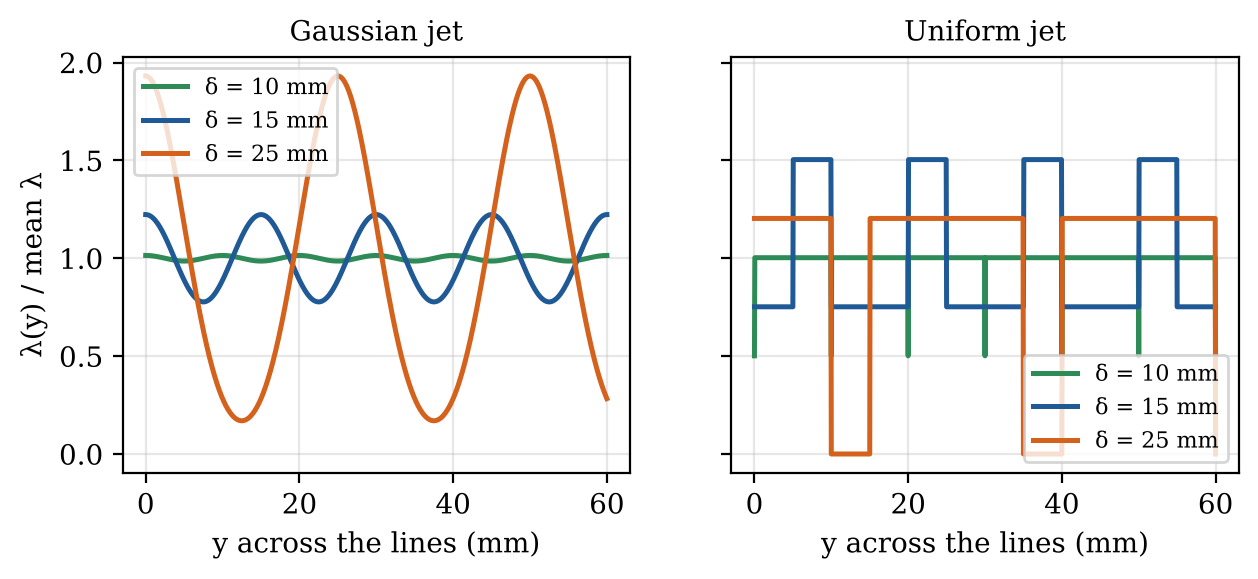
\includegraphics[width=0.92\linewidth]{img/stripes.png}
\caption{Impacts per point across the lines for one raster, divided by the mean, for $\dX=\SI{20}{mm}$. Gaussian jet: smooth stripes whose amplitude grows quickly above $\delta=\dX/2$. Uniform jet: steps between $m_0$ and $m_0+1$ crossings; no stripes for $\delta=\SI{10}{mm}$ ($\dX/\delta=2$), untreated strips for $\delta=\SI{25}{mm}>\dX$.}
\label{fig:stripes}
\end{figure}

\paragraph{Flattened Gaussian and the general rule.} The stripes are set by the Fourier transform $\hat g$ of the profile: the sum over the lines has harmonics of amplitude $2\hat g(k/\delta)/\delta$, so the first harmonic gives a peak-to-peak amplitude $\simeq4\,|\hat g(1/\delta)|$. For the Gaussian, $\hat g$ is itself a positive Gaussian, which gives the formula above. For the uniform jet, $\hat g$ is a sinc function, which vanishes for $\delta=\dX/m$: these are the steps without stripes. The flattened Gaussian has no closed form, and its transform oscillates around zero like the sinc, so its stripes vary with $\delta$ in a non-monotonic way (Fig.~\ref{fig:stripesp}). With $\dX=\SI{20}{mm}$ and $p=4$, the stripes are \SI{6.2}{\percent} at $\delta=\SI{15}{mm}$ against \SI{44.6}{\percent} for the Gaussian, but \SI{32.4}{\percent} at $\delta=\SI{10}{mm}$ against \SI{2.9}{\percent}. A flatter profile is therefore not always worse: the stripes depend on both $p$ and $\delta$, and the page computes them numerically.

\begin{figure}[H]
\centering
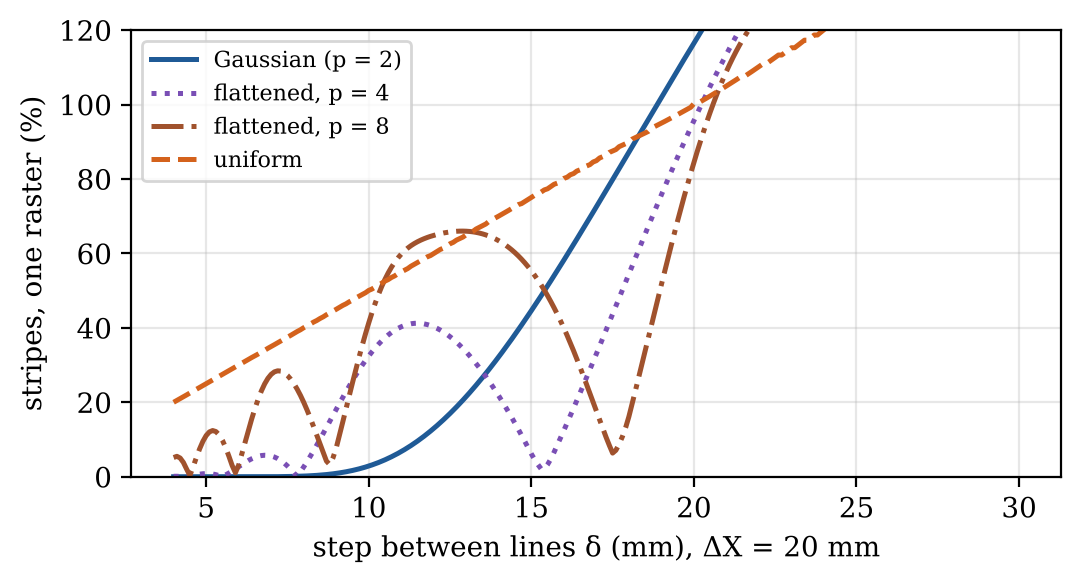
\includegraphics[width=0.66\linewidth]{img/stripes_p.png}
\caption{Stripe amplitude $(\lambda_{\max}-\lambda_{\min})/\bar\lambda$ of one raster versus the step, for $\dX=\SI{20}{mm}$. The flattened profiles oscillate between the Gaussian and the uniform curves. For the uniform jet the amplitude is $\delta/\dX$ except exactly at $\delta=\dX/m$, where it drops to zero.}
\label{fig:stripesp}
\end{figure}

\paragraph{Half-step offset.} Shifting every other raster by $\delta/2$ doubles the spatial frequency of the stripes, which is equivalent to halving the step for the pairs of rasters. With a Gaussian jet and $\delta=\SI{15}{mm}$ the stripes fall from \SI{44.6}{\percent} to \SI{0.1}{\percent}.

\begin{figure}[H]
\centering
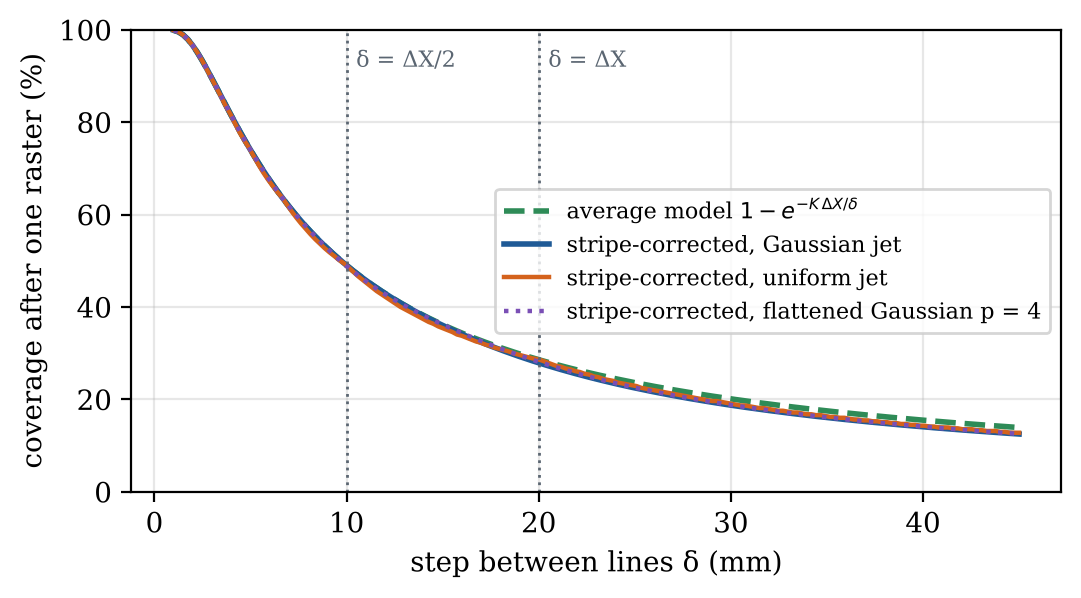
\includegraphics[width=0.66\linewidth]{img/cov_delta.png}
\caption{Coverage after one raster versus the step $\delta$ (default parameters). The stripe-corrected curves fall below the average model as soon as stripes appear; the uniform jet joins it whenever $\dX/\delta$ is a whole number.}
\label{fig:cdelta}
\end{figure}

\section{Crossed rasters at 0° and 90°}

The 0° rasters make stripes along $y$, the 90° rasters along $x$. Over a square cell of side $2\delta$, $x$ and $y$ vary independently, so the mean of $e^{-\lambda}=e^{-\lambda_0(y)}\,e^{-\lambda_{90}(x)}$ factorises and gives Eq.~\eqref{eq:corr}. In the page, $\lambda_0$ and $\lambda_{90}$ are built from the one-raster profiles without offset ($A$) and with the half-step offset ($B$): $n_0$ rasters at 0° give $\lambda_0=\lceil n_0/2\rceil A+\lfloor n_0/2\rfloor B$, and likewise for 90°. Only the numbers $n_0$ and $n_{90}$ matter for the final coverage; the order changes the intermediate states.

\paragraph{Crossing never reduces coverage.} Without offset, $\lambda_0=n_0\,\ell(y)$ and $\lambda_{90}=n_{90}\,\ell(x)$, where $\ell$ is the profile of one raster. For $n=n_0+n_{90}$ rasters all at 0°, the uncovered fraction is $\langle e^{-n_0\ell}\,e^{-n_{90}\ell}\rangle$. Both factors decrease with $\ell$, so by Chebyshev's sum inequality
\begin{equation}
\bigl\langle e^{-n_0\ell}\,e^{-n_{90}\ell}\bigr\rangle\;\ge\;\bigl\langle e^{-n_0\ell}\bigr\rangle\,\bigl\langle e^{-n_{90}\ell}\bigr\rangle .
\end{equation}
The left side is the uncovered fraction of parallel passes, the right side that of crossed passes: for the same number of rasters, crossing gives at least as much coverage. In parallel passes the weak stripes always fall on the same weak stripes; in crossed passes they fall across the strong stripes of the other direction, and the stripes become a finer checkerboard (Fig.~\ref{fig:maps}). The weakest point, where two weak stripes cross, keeps the same $\lambda_{\min}$, so the minimum coverage does not change. The average model only sees the total $n$ and cannot distinguish the two cases.

\begin{figure}[H]
\centering
\begin{subfigure}{0.46\linewidth}\centering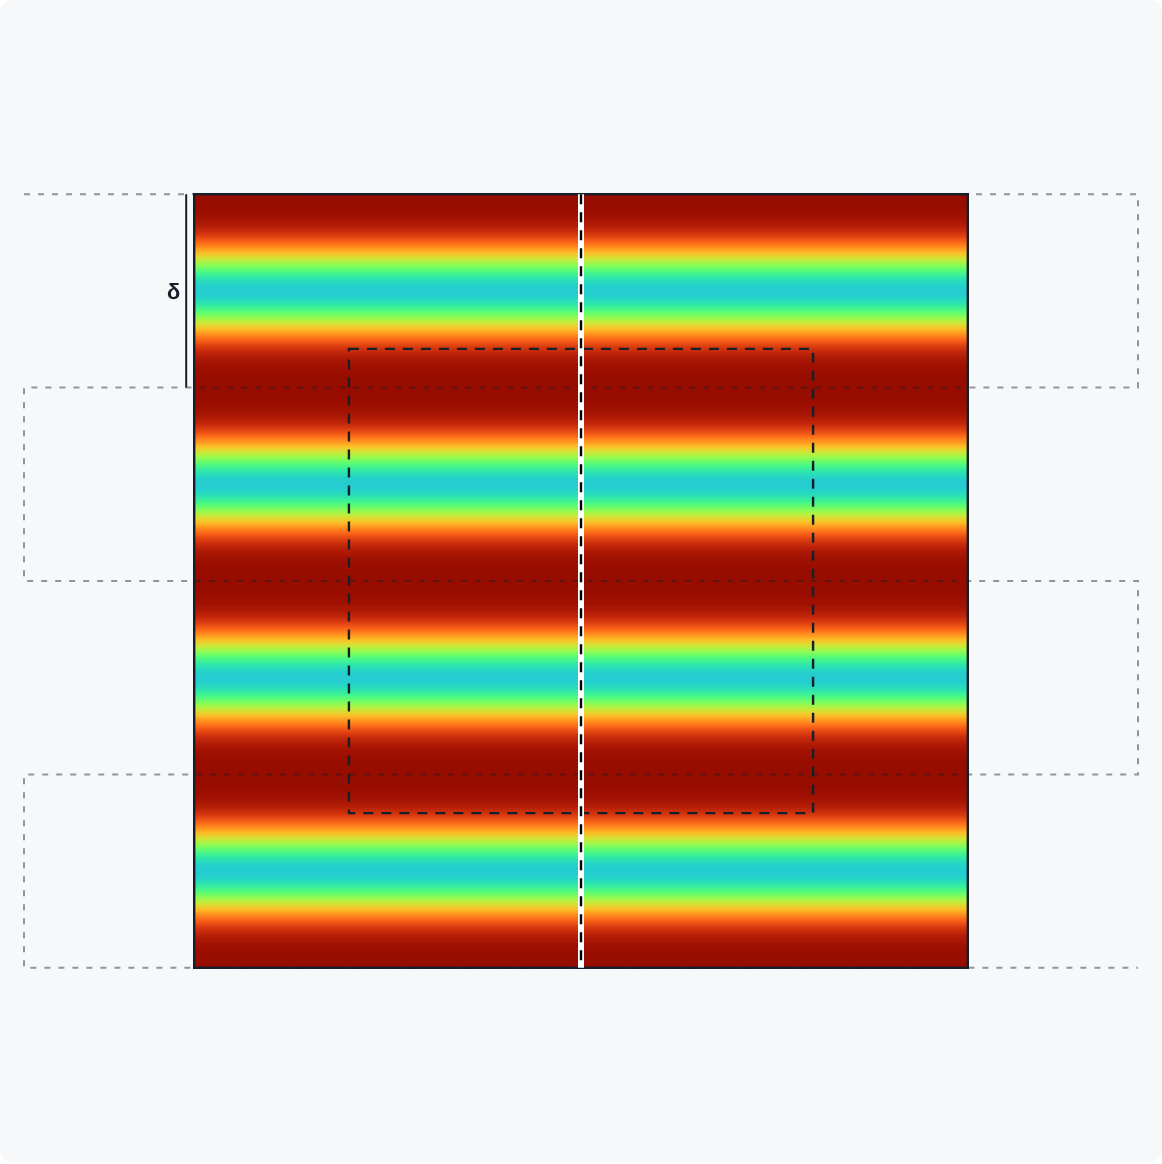
\includegraphics[width=\linewidth]{img/map_par25.png}\caption{6 rasters at 0°: 72.7 \% (simulation)}\end{subfigure}\hfill
\begin{subfigure}{0.46\linewidth}\centering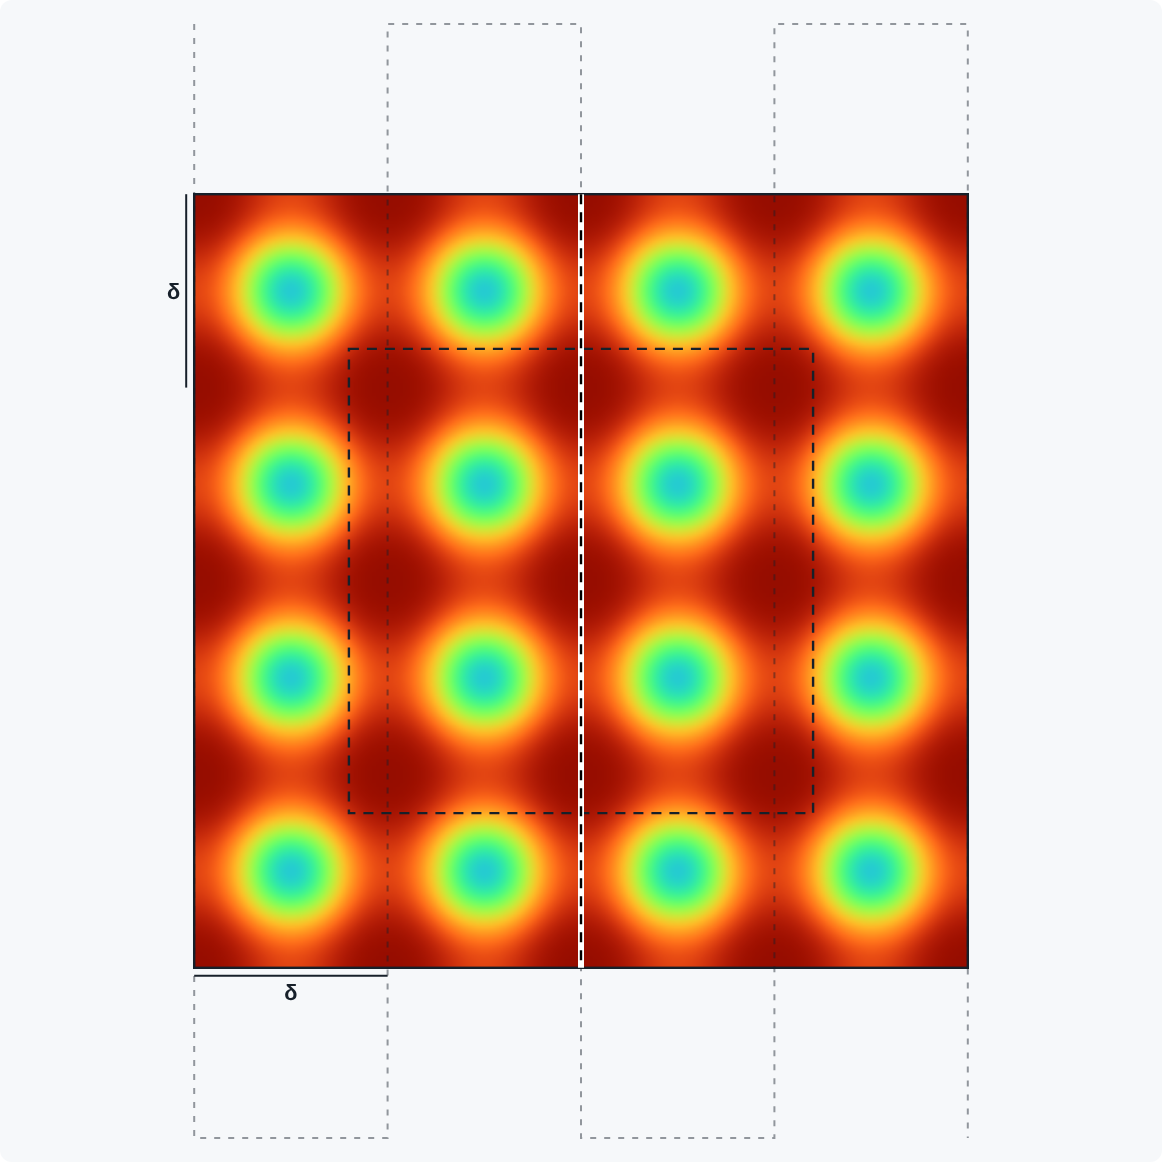
\includegraphics[width=\linewidth]{img/map_cross25.png}\caption{3 at 0° + 3 at 90°: 78.4 \% (simulation)}\end{subfigure}
\caption{Coverage maps of a \SI{100}{mm} part with a Gaussian jet, $\dX=\SI{20}{mm}$ and a large step $\delta=\SI{25}{mm}$, after 6 rasters. Same number of rasters, same time; crossing turns the stripes into a checkerboard and raises the mean coverage. The dashed square is the central zone used for the statistics.}
\label{fig:maps}
\end{figure}

\begin{figure}[H]
\centering
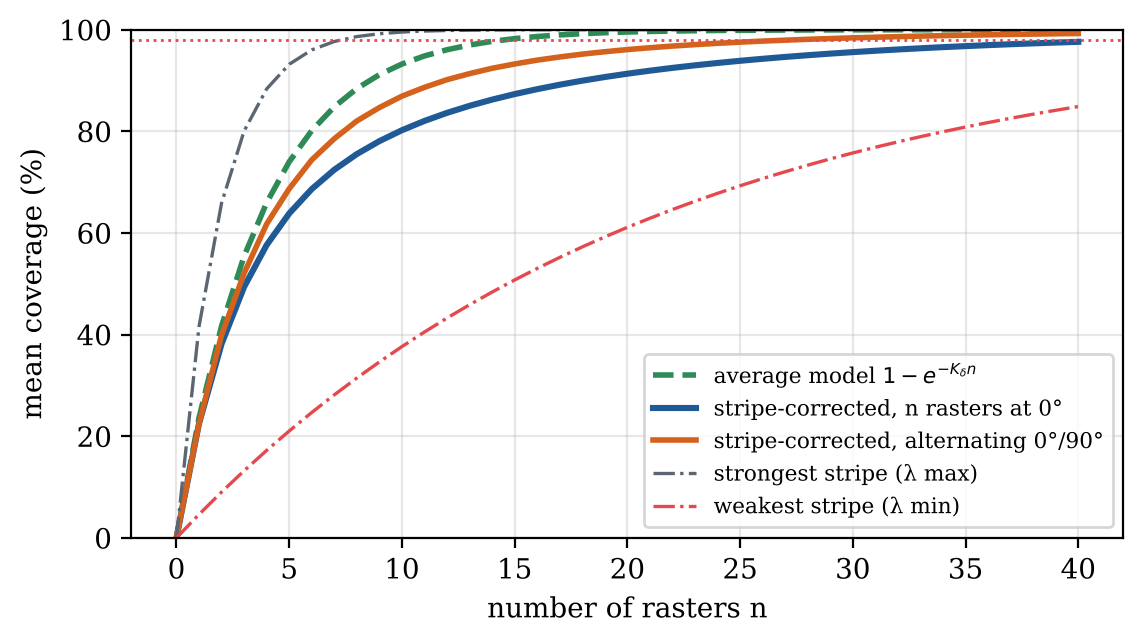
\includegraphics[width=0.74\linewidth]{img/cov_n.png}
\caption{Mean coverage versus the number of rasters for $\delta=\SI{25}{mm}$ (Gaussian jet, default parameters). The average model is an upper bound. The stripe-corrected mean lies between the coverage of the weakest stripe and that of the strongest stripe. For an infinitely large part (mean over whole periods, as plotted), alternating 0° and 90° rasters reaches \SI{98}{\percent} in 27.4 rasters instead of 43.0 for parallel passes; the average model predicts 14.5. On the $100\times\SI{100}{mm}$ part of the page: 23.4 and 39.9 rasters.}
\label{fig:cn}
\end{figure}

\section{Where is the randomness?}

The Shot Peening Coverage Simulator draws every shot at a random position, so each run gives a different set of dents. The extended simulator draws no random numbers: running it twice with the same parameters gives the same map. This is intended, and the randomness is not lost:
\begin{itemize}[leftmargin=*]
\item The page computes the \emph{expected} number of impacts per point $\lambda(x,y)$ (a mean-field calculation).
\item If impacts land at random, independent positions, the number of impacts at a point follows a Poisson law of mean $\lambda$: $P(k)=e^{-\lambda}\lambda^k/k!$. The uncovered fraction is $P(0)=e^{-\lambda}$, which is exactly why $\tau=1-e^{-\lambda}$. The formula used at each point is therefore the expected coverage of a random dent pattern.
\item At the scale of a part the fluctuations around this expectation are negligible. With $r=\SI{10}{\micro m}$, one dent covers \SI{3.1e-4}{mm^2}; $\lambda\approx2.6$ means about \num{8000} dents per square millimetre and tens of millions on a $100\times\SI{100}{mm}$ part. One map cell ($\approx0.45\times\SI{0.45}{mm}$) holds about \num{1600} dents, so its covered fraction would vary by about \SI{1}{\percent} between random runs, and the mean over the central zone by less than \SI{0.01}{\percent}.
\end{itemize}
Randomness is visible at the scale of the dents (first simulator) and averages out at the scale of the part (extended simulator). The stripes are a deterministic effect of the path; they are the same on every run. Not modelled in either simulator are process fluctuations such as variations of the flow rate, of the speed or of the jet position.

\section{Algorithm}

\paragraph{Grid.} The part is divided into about $220$ cells along its longer side (cell size $h=\max(W,H)/220$). The array $\lambda_{ij}$ starts at zero.

\paragraph{Deposition.} When the nozzle moves from $s_0$ to $s_1$ along a line (constant speed), the impacts are added cell by cell with exact integrals rather than random draws:
\begin{itemize}[leftmargin=*]
\item across the line, the weight of cell $j$ is the average of $g$ over the cell, $[G(y_{j+1}-y_c)-G(y_j-y_c)]/h$, where $G$ is the cumulative of $g$ (an error function for the Gaussian jet, a regularised incomplete gamma function $P$ for the flattened Gaussian: $G(u)=\tfrac12+\tfrac12\,\mathrm{sign}(u)\,P\bigl(1/p,\,|u/w|^p\bigr)$);
\item along the line, the weight of cell $i$ is the integral of the footprint over all nozzle positions between $s_0$ and $s_1$, computed with the integral of the cumulative $I(u)=\int_{-\infty}^u G(v)\,\mathrm{d}v$:
\begin{equation}
\omega_i=\frac{I(x_{i+1}-s_0)-I(x_{i+1}-s_1)-I(x_i-s_0)+I(x_i-s_1)}{h}.
\end{equation}
\end{itemize}
For the flattened Gaussian, integrating by parts gives
\begin{equation}
I(u)=u\,G(u)+\frac{w\,\Gamma(2/p)}{2\,\Gamma(1/p)}\,Q\bigl(2/p,\,|u/w|^p\bigr),
\end{equation}
where $Q=1-P$; the incomplete gamma functions are evaluated by their series and continued-fraction expansions. Each cell receives $\frac{a\dot N}{V}\,\omega_i\,\omega_j$. The result does not depend on the animation speed or on the time step: \textsf{Run all} and the animation give identical maps.

\paragraph{Statistics.} The mean, minimum and maximum coverage are computed over the central zone, at a distance $\dX$ from the edges. The stripe amplitude is $(\lambda_{\max}-\lambda_{\min})/\bar\lambda$ in this zone.

\paragraph{Rasters and time to reach 98 \%.} For the stripe-corrected model, the page repeats the chosen sequence of rasters if needed, finds the first whole number of rasters $k$ with $\bar\tau\ge\SI{98}{\percent}$ and interpolates linearly between $k-1$ and $k$. For the average model, $n_{98}=\ln 50/K_\delta$. The time of one raster is (number of lines)$\times$(line length $+$ 2 overtravels)$/V$, computed separately for 0° and 90° rasters.

\section{Validation}

Table~\ref{tab:valid} compares the mean coverage in the central zone of the simulated map with the stripe-corrected model, computed independently in Python, and with the average model.

\begin{table}[H]
\centering\small
\caption{Validation with the default parameters ($K=0.337$, $\dX=\SI{20}{mm}$, $W=H=\SI{100}{mm}$) unless stated.}
\label{tab:valid}
\setlength{\tabcolsep}{4pt}
\begin{tabular}{@{}lccccc@{}}
\toprule
Jet & $\delta$ (mm) & Rasters & Simulation & Stripe-corrected & Average model\\
\midrule
Uniform & 20 & 1 at 0° & 28.6 \% & 28.6 \% & 28.6 \%\\
Uniform & 15 & 1 at 0° & 35.4 \% & 35.4 \% & 36.2 \%\\
Uniform & 10 & 1 at 0° & 49.0 \% & 49.0 \% & 49.0 \%\\
Uniform & 8 & 1 at 0° & 56.3 \% & 56.3 \% & 56.9 \%\\
Uniform & 5 & 1 at 0° & 74.0 \% & 74.0 \% & 74.0 \%\\
Gaussian & 15 & 6 at 0° & 92.6 \% & 92.6 \% & 93.2 \%\\
Gaussian & 15 & 3 + 3, alternate & 92.9 \% & 92.9 \% & 93.2 \%\\
Gaussian & 15 & 3 + 3, 0° first & 92.9 \% & 92.9 \% & 93.2 \%\\
Uniform & 15 & 2 + 2, alternate & 81.8 \% & 81.8 \% & 83.4 \%\\
Gaussian & 15 & 4 + 2, half-step offset & 93.2 \% & 93.2 \% & 93.2 \%\\
\midrule
Gaussian & 25 & 6 at 0° & 72.7 \% & 72.7 \% & 80.1 \%\\
Gaussian & 25 & 3 + 3, alternate & 78.4 \% & 78.4 \% & 80.1 \%\\
\midrule
Flattened, $p=2$ & 15 & 6 at 0° & 92.6 \% & 92.6 \% & 93.2 \%\\
Flattened, $p=4$ & 15 & 6 at 0° & 93.2 \% & 93.2 \% & 93.2 \%\\
Flattened, $p=4$ & 10 & 6 at 0° & 98.0 \% & 98.0 \% & 98.2 \%\\
Flattened, $p=4$ & 15 & 3 + 3, half-step offset & 93.2 \% & 93.2 \% & 93.2 \%\\
Flattened, $p=20$ & 10 & 1 at 0° & 48.9 \% & 48.9 \% & 49.0 \%\\
Flattened, $p=20$ & 15 & 1 at 0° & 35.6 \% & 35.6 \% & 36.2 \%\\
Flat., $p=3$, $\dX=\SI{30}{mm}$ & 12 & 2 + 2, part 150 × 120 & 89.4 \% & 89.4 \% & 89.4 \%\\
Flattened, $p=4$ & 25 & 3 + 3, alternate & 78.1 \% & 78.1 \% & 80.1 \%\\
\bottomrule
\end{tabular}
\end{table}

For the default case (Gaussian, $\delta=\SI{15}{mm}$, 6 rasters at 0°) the simulated stripes are \SI{44.5}{\percent} against \SI{44.6}{\percent} predicted, with a local coverage between \SI{87.7}{\percent} and \SI{96.3}{\percent}; \SI{98}{\percent} is reached in 9.2 rasters (8.7 with the average model).

The simulated map and the stripe-corrected model agree in every case, and both agree with an independent Python computation (mean, minimum and maximum coverage, stripe amplitude and $n_{98}$), including the tilted nozzles ($\theta$, $\psi$) and two nozzles. Since version 2.2 the model is averaged over the central zone of the part rather than over one period of the stripes. The two differ when the zone does not contain a whole number of periods: for $\delta=\SI{25}{mm}$ the zone (\SI{60}{mm}) covers 2.4 periods and contains more strong stripes than weak ones, so the part shown reaches 78.4\,\% after the 6 rasters and 98\,\% after 23.4 rasters, whereas an infinitely large part would reach 74.4\,\% and need 27.4 rasters. The model now describes the part on the screen, so the base time, the times for full and specified coverage and the coverage (NF~L~06-832) are consistent with the map.


\section{Every parameter}\label{sec:params}

\begin{longtable}{@{}p{3.6cm}p{1.4cm}p{2.0cm}p{1.6cm}p{4.9cm}@{}}
\toprule
\textbf{Parameter} & \textbf{Unit} & \textbf{Range} & \textbf{Default} & \textbf{Effect}\\ \midrule\endhead
Media flow rate $\dot m$ (per nozzle) & kg/min & 0.1 -- 6 & 1.5 & $\lambda\propto\dot m$.\\
Media density $\rho$ & g/cm³ & 1 -- 8 & 2.2 & $\lambda\propto1/\rho$ at fixed flow rate.\\
Mass median diameter $D_{50}$ & µm & 30 -- 1000 & 150 & Number of shots per second $\propto1/D_{50}^3$.\\
Size spread $\sigma$ & -- & 0 -- 0.6 & 0 & Log-normal spread of the shot sizes.\\
Dent radius $r$ (for $D_{50}$) & µm & 2 -- 100 & 10 & Dent area $a\propto r^2$.\\
Jet size $\dX$ & mm & 2 -- 60 & 20 & Width of the jet; sets the overlap $\dX/\delta$ and the stripes. It does not change the mean $\lambda$.\\
Jet profile & -- & 3 choices & Gaussian & Uniform, Gaussian ($\sigma_j=\dX/4$) or flattened Gaussian; the \ui{i} button opens the page ``Jet Profile Explained''.\\
Flatness exponent $p$ & -- & 2 -- 20 & 4 & Only for the flattened Gaussian; 2 = Gaussian, large = uniform.\\
Traverse speed $V$ & mm/s & 10 -- 2000 & 300 & $\lambda\propto1/V$; also sets the time of a raster.\\
Number of nozzles & -- & 1 or 2 & 1 & Same plane, aimed at the same point; $\dot m$ per nozzle.\\
Angle $\theta_1$ of nozzle 1 & ° & 0 -- 60 & 0 & 0 = normal; tilt in the plane (path, normal). $\lambda\propto f(\theta)$; stripes unchanged; longer overtravel.\\
Angle $\theta_2$ of nozzle 2 & ° & $-60$ -- 0 & 0 & Tilted the other way; only with 2 nozzles.\\
Angle $\psi$ of the nozzle plane & ° & 0 -- 60 & 0 & Tilt across the path; jet $\dX/\cos\psi$ wide across the lines: smoother stripes.\\
Dent area at angle $\theta$ & -- & 2 choices & $\cos\theta$ & $f(\theta)=\cos\theta$ or $\cos^2\theta$ (Section~\ref{sec:tilt}).\\
Step between lines $\delta$ & mm & 0.5 -- 80 & 15 & $\lambda\propto1/\delta$; stripes when $\delta$ is large compared with $\dX$.\\
Rasters at 0° & -- & 0 -- 30 & 3 & Rasters of horizontal lines (along $x$).\\
Rasters at 90° & -- & 0 -- 30 & 3 & Rasters of vertical lines (along $y$).\\
Order of the rasters & -- & 2 choices & alternate & 0°, 90°, 0°, 90°\ldots or all 0° first. Changes the intermediate states, not the final map.\\
Offset between rasters & -- & 2 choices & none & ``Half step'' shifts every other raster of the same direction by $\delta/2$.\\
Part length $W$, width $H$ & mm & 20 -- 400 & 100 & Size of the part; sets the number and length of the lines.\\
Specified coverage $C$ & \% & 50 -- 500 & 100 & Used for the number of rasters and the time (Section~\ref{sec:above}); does not restart the simulation.\\
Full coverage (100\,\%) & -- & 2 choices & 1.25 × base & NF~L~06-832 factor 1.25, or 100\,\% = base time.\\
\bottomrule
\end{longtable}
\noindent At least one raster is always kept. Changing a physical parameter restarts the simulation; \ui{Reset to default values} restores the defaults.

\section{Every result displayed}\label{sec:reads}

\begin{longtable}{@{}p{4.4cm}p{7.2cm}p{2.0cm}@{}}
\toprule
\textbf{Readout} & \textbf{Meaning and formula} & \textbf{Default}\\ \midrule\endhead
\ui{Rasters done} & completed rasters / planned rasters & 6 / 6\\
\ui{Order of the rasters} & the planned sequence of directions & 0°·90°·…\\
\ui{Overlap ratio ΔX/δ} & mean number of lines crossing a point per raster & 1.33\\
\ui{Mean coverage (central zone)} & mean of $1-e^{-\lambda}$ over the zone at a distance $\dX$ from the edges & 92.9\,\%\\
\ui{Min / max coverage} & weakest and strongest point of that zone & 87.7 / 96.3\,\%\\
\ui{Mean impacts per point λ} & mean of $\lambda$ in the zone & 2.69\\
\ui{Stripe amplitude} & $(\lambda_{\max}-\lambda_{\min})/\bar\lambda$ in the zone & 44.5\,\%\\
\ui{Average model} & $100(1-e^{-K_\delta n})$, $n$ = all planned rasters & 93.2\,\%\\
\ui{Stripe-corrected model} & Eq.~\eqref{eq:corr} for the planned rasters & 92.9\,\%\\
\ui{Coverage (NF L 06-832)} & mean dented area up to $t_b$, then time-based; time counted as $\bar\lambda/K_\delta$ rasters (Section~\ref{sec:above}) & 92.9\,\%\\
\ui{Min / max coverage (NF L 06-832)} & local coverage $C(x,y)$ of the weakest and strongest point (Section~\ref{sec:above}) & 87.7 / 96.3\,\%\\
\ui{Rasters for 98\,\% = base time} & stripe-corrected model, plan repeated if needed & 8.9\\
\ui{Rasters for 98\,\% (average model)} & $\ln50/K_\delta$ & 8.7\\
\ui{Lines per raster 0° / 90°} & number of lines of one raster & 7 / 7\\
\ui{Time per raster 0° / 90°} & lines × (line length + 2 overtravels) / $V$ & 3.4 s\\
\ui{Time for the planned rasters} & sum over the plan & 20.2 s\\
\ui{Time to reach 98\,\% (base time)} & time of $n_{98}$ rasters & 30.0 s\\
\ui{Rasters for 100\,\% = 1.25 × base} & $1.25\,n_{98}$, with its time & 11.2 (37.5 s)\\
\ui{Rasters / Time for C} & inverse of $C(t)$; $\frac{C}{100}\times1.25\,n_{98}$ above 100\,\% & 11.2, 37.5 s\\
\bottomrule
\end{longtable}

\noindent The calculation chain lists $\E[D^3]$ (with its equivalent diameter), $\dot N$, $a$, $K$, $K_\delta$, the mean $\lambda$, the stripe-corrected coverage, the stripe amplitude of one raster with its formula for the current profile, the time of full coverage, and the effect of crossing (coverage of the plan compared with all the rasters at 0°). Hovering over the map gives $\lambda$, $\tau$ and the local coverage (NF~L~06-832) at the pointer.

\section{Coverage above 100\,\% (NF~L~06-832)}\label{sec:above}

NF~L~06-832 defines the \textbf{base time} $t_b$ as the time needed to reach 98\,\% coverage, \textbf{full coverage (100\,\%)} as $1.25\,t_b$, and a coverage of $C$\,\% as $\frac{C}{100}\times1.25\,t_b$: 200\,\% is twice the time of full coverage. On the page:
\begin{itemize}[leftmargin=*]
\item the base time comes from the stripe-corrected model, as an inspector would measure it on the real, striped part: $n_{98}$ rasters;
\item full coverage needs $1.25\,n_{98}$ rasters, and the specified coverage $C$ needs $\frac{C}{100}\times1.25\,n_{98}$;
\item on an even treatment, full coverage corresponds to $\lambda_{100}=1.25\ln50=4.89$ impacts per point (99.25\,\% dented).;
\item with the option \ui{= base time}, the factor 1.25 is dropped: $\lambda_{100}=\ln 50=3.91$ and 100\,\% means 98\,\% dented.
\end{itemize}
\paragraph{The readout \ui{Coverage (NF L 06-832)}.} Coverage is the dented area divided by the total area as long as it can be measured, i.e.\ up to 98\,\%. Beyond, NF~L~06-832 counts time. The page combines both in one value, $C(t)$, continuous and increasing:
\begin{equation}
C(t)=\begin{cases}
\text{dented area (\%)} & t\le t_b\quad(\text{reaches }98\,\%\text{ at }t_b)\\[2pt]
98+2\,\dfrac{t/t_b-1}{0.25} & t_b<t\le1.25\,t_b\quad(98\to100\,\%)\\[6pt]
100\,\dfrac{t}{1.25\,t_b} & t>1.25\,t_b
\end{cases}
\end{equation}
With the option \ui{Full coverage (100\,\%) = base time}, the middle interval disappears: $C=100\,t/t_b$ after the base time. The number of passes (or the time) for a specified coverage $C$ is the inverse of this function: below 98\,\% it comes from the dented area, above 100\,\% it is $\frac{C}{100}\times1.25\,t_b$.

\begin{center}\small
\begin{tabular}{@{}lccccccc@{}}
\toprule
Passes $n$ (reference case, $K=0.337$) & 1 & 3 & 6 & 11.6 ($t_b$) & 13.0 & 14.5 & 29.0\\ \midrule
Dented area (\%) & 28.6 & 63.6 & 86.8 & 98.0 & 98.8 & 99.25 & 99.99\\
Coverage (NF L 06-832) (\%) & 28.6 & 63.6 & 86.8 & 98 & 99 & 100 & 200\\ \bottomrule
\end{tabular}
\end{center}

\paragraph{Local coverage of a point.} On the flat-part and cylinder simulators the same rule is applied to each point, with time replaced by the number of impacts it has received (proportional to time on an even treatment): $C(x,y)=1-e^{-\lambda}$ up to $\lambda=\ln50=3.91$ (98\,\%), then 98 to 100\,\% up to $\lambda=1.25\ln50=4.89$, and $100\,\lambda/4.89$ above. The hover readout gives it, and the map can show it (\ui{Map shows: coverage NF L 06-832}).


\noindent With the defaults, 12 rasters give a mean dented area of 99.5\,\% (98.5 to 99.9\,\%) and a coverage (NF~L~06-832) of 107\,\% (98.6 to 135\,\% from the weakest to the strongest point).

\textbf{Stripes lengthen the base time.} On a striped part the weak stripes are the last to be dented, so the base time is longer than on an even one: with the defaults $n_{98}=8.9$ rasters instead of 8.7 for the average model, and 23.4 instead of 14.5 with $\delta=\SI{25}{mm}$. The fraction of a raster is exact on a flat part: it stands for a raster with the same path at a proportionally lower speed.

\section{Tilted nozzle}\label{sec:tilt}

The nozzle can be tilted by an angle $\theta$ (0 to 60°, 0 = normal to the surface) in the plane that contains the path of the nozzle and the normal to the surface. Two things change.

\paragraph{The footprint gets longer, not wider.} A jet of width $\dX$ meets the surface obliquely: its footprint is $\dX/\cos\theta$ long along the path and still $\dX$ wide across it. The flow per unit area under the footprint drops by $\cos\theta$, but a point stays under the jet $1/\cos\theta$ times longer. The swept width is still $\dX$, so the number of shots per unit area in one pass is unchanged:
\begin{equation}
R=\frac{\dot N}{V\,\dX}\quad\text{(independent of }\theta\text{)},\qquad \text{time under the jet } \frac{\dX}{V\cos\theta}.
\end{equation}
The centre of the footprint is also shifted along the path by $d\tan\theta$ ($d$: stand-off distance). This constant shift moves the whole pattern; it does not change the coverage inside the part.

\paragraph{Each dent is smaller.} Only the normal component of the shot velocity, $v_n=v\cos\theta$, indents the surface; the tangential component makes the dent slightly oval and causes some sliding, which the model does not draw. The dent area is multiplied by a factor $f(\theta)$, chosen with the parameter \ui{Dent area at angle θ}:
\begin{equation}
a(\theta)=a_0\,f(\theta),\qquad f(\theta)=\cos\theta\ \ (\text{dent radius}\propto\sqrt{v_n})\quad\text{or}\quad f(\theta)=\cos^2\theta\ \ (\text{normal kinetic energy}),
\end{equation}
where $a_0$ is the dent area at normal incidence (the parameter \ui{Dent radius r} is the radius at normal impact). Measurements usually fall between the two laws. The rate constant becomes $K(\theta)=K_0\,f(\theta)$, and all the times (98\,\%, full coverage, specified coverage) are multiplied by $1/f(\theta)$:

\begin{center}\small
\begin{tabular}{@{}lcccc@{}}
\toprule
$\theta$ & 15° & 30° & 45° & 60°\\ \midrule
time factor, $f=\cos\theta$ & 1.04 & 1.15 & 1.41 & 2.00\\
time factor, $f=\cos^2\theta$ & 1.07 & 1.33 & 2.00 & 4.00\\ \bottomrule
\end{tabular}
\end{center}

\noindent Not modelled: the oval shape of the dents, the lower peening intensity, the fewer collisions between incoming and rebounding shots (which can partly compensate up to about 20--30°), and the grazing impacts at large angles.

\subsection*{Two nozzles}

The parameter \ui{Number of nozzles} adds a second nozzle in the same plane, aimed at the same point and tilted the other way: nozzle~1 at $\theta_1\ge0$, nozzle~2 at $\theta_2\le0$. Each nozzle throws the flow rate $\dot m$ (the parameter is per nozzle). The two jets act independently: their impacts add up, $\lambda=\lambda_1+\lambda_2$, and since each one follows the rules above,
\begin{equation}
K=K_0\,\bigl[f(\theta_1)+f(\theta_2)\bigr],
\end{equation}
where $K_0$ is the rate constant of one nozzle at normal incidence. Two normal nozzles ($\theta_1=\theta_2=0$) are exactly one nozzle with twice the flow rate; two nozzles at $\pm45°$ give $1.41\,K_0$ (law $\cos\theta$) or $1.00\,K_0$ (law $\cos^2\theta$): with the $\cos^2\theta$ law, two nozzles at $\pm45°$ do the work of one normal nozzle. The coverage does not depend on the signs of the angles, only on $f(\theta_1)+f(\theta_2)$ and on the footprint lengths $\dX/\cos\theta_1$ and $\dX/\cos\theta_2$. What two opposite nozzles do change in practice, and the model does not include, is the symmetry of the treatment: the tangential components of the two jets are opposite, so the asymmetric pile-up and the directional effects of a single oblique jet tend to cancel. Collisions between the two streams near the surface are not modelled either.

\subsection*{Angle \texorpdfstring{$\psi$}{psi} across the path}

The angle $\psi$ (0 to 60°) tilts the plane of the nozzle (or of the two nozzles) about the direction of the path. With $\theta$ measured in that plane, the axis of a nozzle, pointing from the surface to the nozzle, is
\begin{equation}
\mathbf a=(\sin\theta,\ \cos\theta\sin\psi,\ \cos\theta\cos\psi)\quad(x\text{ along the path},\ y\text{ across it},\ z\text{ along the normal}),
\end{equation}
so the angle of incidence $\gamma$ is given by $\cos\gamma=\cos\theta\cos\psi$, and the dent area is multiplied by $f(\gamma)=\cos\gamma$ or $\cos^2\gamma$. A jet of width $\dX$ projected along $\mathbf a$ on the surface has a footprint (exact for a Gaussian jet, used for all the profiles)
\begin{equation}
\text{across the path: } \frac{\dX}{\cos\psi},\qquad \text{along the path: } \dX\sqrt{1+\frac{\tan^2\theta}{\cos^2\psi}} .
\end{equation}
The width across the path does not depend on $\theta$, and the length along it reduces to $\dX/\cos\theta$ when $\psi=0$. The consequences differ between the simulators:
\begin{itemize}[nosep,leftmargin=*]
\item \textbf{one line swept again and again} (Shot Peening Coverage Simulator): the swept width grows to $\dX/\cos\psi$, so the impacts per unit area and per pass drop by $\cos\psi$: $K=K_0\cos\psi\sum_k f(\gamma_k)$;
\item \textbf{raster on a flat part}: the mean number of impacts per raster does not depend on the width of the jet, only $f(\gamma)$ changes it; but the wider jet overlaps more lines ($\dX/(\delta\cos\psi)$), which \emph{smooths the stripes};
\item \textbf{cylinder}: the jet no longer aims at the axis. In the cross-section, the ray at a lateral offset $u$ from the jet axis hits the surface at the arc length $s$ given by $u(s)=R\,[\sin(s/R+\psi)-\sin\psi]$; the flux on the surface becomes $g_s(s)=g(u(s))\cos(s/R+\psi)$ for $|s/R+\psi|<\pi/2$, the share of the shots that hit the cylinder becomes $c=G(R(1-\sin\psi))-G(-R(1+\sin\psi))$, and the footprint around the circumference gets longer and asymmetric. With the curvature ignored, $g_s(s)=g(s\cos\psi)\cos\psi$.
\end{itemize}
New views show the angles: the side view along the path shows $\theta_1$, $\theta_2$, and a front view across the path shows $\psi$ (Shot Peening Coverage Simulator and flat part); on the cylinder a cross-section perpendicular to the axis shows the nozzle tilted by $\psi$, its jet, the treated arc of the circumference and the shots that miss. With two nozzles, both lie in the plane tilted by $\psi$, so they appear as one nozzle in the front view or cross-section. The nozzles keep their orientation relative to the path (on the flat part they turn with the 0° and 90° rasters).


\noindent On the flat part, the profile of the jet across the lines, the overlap $\dX/\delta$ and the stripes do not change: only $\lambda$ is multiplied by $f(\theta)$. The footprint drawn on the map is $\dX/\cos\theta$ long along the current line, and the overtravel beyond the part ends grows in the same ratio, which makes each raster slightly longer. With $\theta=45°$ and $f=\cos\theta$: mean coverage 84.8\,\% (77.3 to 90.2\,\%) instead of 92.9\,\% (87.7 to 96.3\,\%), and 12.6 rasters for 98\,\% instead of 8.9 (× 1.41). With $f=\cos^2\theta$: 73.7\,\% and 17.9 rasters.

\noindent With two nozzles at $\pm45°$: mean coverage 97.6\,\% (94.8 to 99.0\,\%) after the 6 rasters, 6.3 rasters for 98\,\% instead of 8.9. The stripes keep the same relative amplitude, since both jets have the same profile across the lines.

\noindent A front view across the current line, under the side view, shows $\psi$, the width of the jet across the path and the neighbouring lines of the raster. With the defaults and $\psi=30°$: mean coverage 90.3\,\% (87.5 to 92.4\,\%), stripe amplitude 21.3\,\% instead of 44.5\,\%, 10.1 rasters for 98\,\% instead of 8.9; at $\psi=60°$ the stripes vanish (0.1\,\%) but the dents are half as large (74.0\,\%, 17.4 rasters).

\section{Things to try}

\begin{center}
\small
\begin{tabular}{@{}lccccl@{}}
\toprule
Change from the defaults & mean $\tau$ & min / max & stripes & $n_{98}$ & Comment\\ \midrule
none (3 + 3, $\delta=15$) & 92.9 & 87.7 / 96.3 & 44.5 & 8.9 & defaults\\
6 at 0°, 0 at 90° & 92.6 & 87.7 / 96.3 & 44.5 & 9.2 & parallel passes\\
$\delta=\SI{10}{mm}$ & 98.2 & 98.1 / 98.3 & 2.8 & 5.8 & no stripes\\
$\delta=\SI{25}{mm}$ & 78.4 & 24.7 / 96.0 & 162 & 23.4 & strong stripes\\
uniform jet & 91.8 & 86.7 / 98.2 & 75.0 & 9.8 & sharp steps\\
flattened jet ($p=4$) & 93.2 & 92.9 / 94.0 & 6.1 & 8.7 & stripes cancel\\
half-step offset & 93.2 & 91.7 / 94.5 & 14.8 & 8.7 & finer stripes\\ \bottomrule
\end{tabular}
\end{center}
\noindent (coverage in \%, stripes = simulated $(\lambda_{\max}-\lambda_{\min})/\bar\lambda$ in \%, $n_{98}$ in rasters.)

\begin{trybox}
\begin{itemize}[nosep,leftmargin=*]
\item Compare \ui{Alternate} and \ui{All 0° first}: the final map is the same, the coverage curve on the way is not.
\item With the uniform jet, try $\delta=20$, 10 and 6.67\,mm ($\dX/\delta=1,2,3$): no stripes at all. In between, steps appear.
\item With the flattened jet, move $p$ and $\delta$: some combinations almost cancel the stripes, others enhance them (Fig.~\ref{fig:stripesp}).
\item Open the jet profile page with the \ui{i} button to see the three profiles and their overlap.
\end{itemize}
\end{trybox}

\section{Assumptions and limits}

Constant traverse speed and flow rate; the jet fires continuously, including during the turnarounds outside the part; flat part and normal incidence; footprint separable in $x$ and $y$; dents proportional to the shot diameter; impacts at independent random positions (Poisson), shown through their expectation. Edge effects of a real part, the angle of incidence, saturation and the variability of the process are not modelled. The model describes how the surface gets covered, not what happens physically beyond full coverage. It does not replace coverage verification according to the applicable standards (NF~L~06-832, SAE~J2277).

\appendix
\section{Symbols}
\begin{tabular}{@{}ll@{\qquad}ll@{}}
$\tau$ & coverage (dented area) & $\lambda$ & expected impacts per point\\
$K$ & dented area per pass along one line & $K_\delta$ & mean dented area per raster, $K\dX/\delta$\\
$a$ & mean dent area & $\dot N$ & shots per second\\
$\delta$ & step between lines & $\dX$ & jet size\\
$g$ & jet profile across the line & $\sigma_j$ & Gaussian width $\dX/4$\\
$p$ & flatness exponent & $w$ & width of the flattened profile\\
$n_0,n_{90}$ & rasters at 0° and 90° & $W,H$ & part length and width\\
$t_b$ & base time (98\,\%) & $C$ & specified coverage\\
$\lambda_{100}$ & impacts per point at 100\,\% & $n_{98}$ & rasters for 98\,\%\\
\end{tabular}

\vfill
\noindent\small Code: MIT licence. Documentation: CC BY 4.0. Related tools: \url{https://rkubler.github.io/shotpeening/}.

\begin{thebibliography}{9}
\bibitem{mt2019} Measurement and functional approximation of peening intensity distributions, \emph{Materials Transactions} 60(6) (2019). \url{https://www.jstage.jst.go.jp/article/matertrans/60/6/60_P-M2019816/_article}
\end{thebibliography}

\end{document}
